\documentclass[12pt, letterpaper]{article}
%\documentclass[12pt, letterpaper, titlepage]{article}

\usepackage{amsmath}
\usepackage{booktabs}
\usepackage{amsthm}
\usepackage{graphicx}
\usepackage[margin=1in]{geometry}
\usepackage{hyperref}
\hypersetup{colorlinks = true, linkcolor = blue, citecolor=blue, urlcolor = blue}
\usepackage{natbib}
\usepackage{enumitem}
\usepackage{setspace}

\usepackage[]{lineno}
\linenumbers*[1]
% %% patches to make lineno work better with amsmath
\newcommand*\patchAmsMathEnvironmentForLineno[1]{%
 \expandafter\let\csname old#1\expandafter\endcsname\csname #1\endcsname
 \expandafter\let\csname oldend#1\expandafter\endcsname\csname end#1\endcsname
 \renewenvironment{#1}%
 {\linenomath\csname old#1\endcsname}%
 {\csname oldend#1\endcsname\endlinenomath}}%
\newcommand*\patchBothAmsMathEnvironmentsForLineno[1]{%
 \patchAmsMathEnvironmentForLineno{#1}%
 \patchAmsMathEnvironmentForLineno{#1*}}%

\AtBeginDocument{%
 \patchBothAmsMathEnvironmentsForLineno{equation}%
 \patchBothAmsMathEnvironmentsForLineno{align}%
 \patchBothAmsMathEnvironmentsForLineno{flalign}%
 \patchBothAmsMathEnvironmentsForLineno{alignat}%
 \patchBothAmsMathEnvironmentsForLineno{gather}%
 \patchBothAmsMathEnvironmentsForLineno{multline}%
}

% control floats
\renewcommand\floatpagefraction{.9}
\renewcommand\topfraction{.9}
\renewcommand\bottomfraction{.9}
\renewcommand\textfraction{.1}
\setcounter{totalnumber}{50}
\setcounter{topnumber}{50}
\setcounter{bottomnumber}{50}

\newcommand{\jy}[1]{\textcolor{blue}{JY: #1}}
\newcommand{\eds}[1]{\textcolor{red}{EDS: (#1)}}
\newcommand{\mc}[1]{\textcolor{green}{MC: (#1)}}

% NOTE: To produce blinded version, replace "0" with "1" below.
\newcommand{\blind}{0}

\begin{document}
%\maketitle

\if0\blind
{
  \title{\bf Nonparametric Bootstrap Kolmogorov-Smirnov Test with Stationary 
  Time Series}
  \author{Mathew Chandy, %\\
%   \href{mailto:mathew.chandy@uconn.edu}
% {\nolinkurl{mathew.chandy@uconn.edu}}\\
  Jun Yan, %\\
  Xianyang Zhang\\
}
\date{}
  \maketitle
} \fi

\if1\blind
{
  \bigskip
  \bigskip
  \bigskip
  \begin{center}
    {\LARGE\bf Nonparametric Bootstrap Kolmogorv-Smirnov Test with Stationary 
    Time Series}
\end{center}
  \bigskip
} \fi


\doublespace

\begin{abstract}

The Kolmogorov-Smirnov (KS) statistic is widely used to test if a sample is
from a given distribution.

\bigskip
\noindent{\sc Keywords}:
\end{abstract}

%\doublespace


\section{Introduction}
\label{sec:intro}

The Kolmogorov-Smirnov (KS) test is a useful goodness-of-fit statistic. It 
can be used to see if a population follows a hypothesized distribution and has 
and can be applied to a variety of fields. It has
been used to analyze the random distribution of cosmic microwave background 
radiation \citep{naess2012application}. A common misuse of the KS test is when
the hypothesized distribution has unspecified parameters. 
\citet{babu2004goodness} approaches this scenario using basic 
non-parametric bootstrap. There is also the scenario where both the hypothesized 
distribution has unspecified parameters and additionally the data are 
serially dependent. \citet{zeimbekakis2022misuses} demonstrates a remedy for
this scenario using semi-parametric bootstrap. This study aims to address this
scenario with non-parametric block bootstrap.


The rest of the paper is outlined as follows: in the first 
section, we assess whether the KS
test holds its size; that is, does the test fail to reject the null hypothesis
when it is true. In the second section, we evaluate the 
test's power; that is, does the test reject the null hypothesis when it is 
false.
Finally, we end with 
concluding remarks in the third section.


\section{Methods}
\label{sec:methods}

Consider a stationary time series $\{X_t: t = 1, \ldots, n\}$ with length~$n$.
\jy{state the null hypothesis explicitly; we are testing the marginal
  distribution. Point out the challenges.}
Let $H_0: X_t ~ F$, where if $F$ is a hypothesized distribution with unknown 
parameters. Let $H_A$ be that $X_t$ does not follow $F$. This is challenging because we are
dealing with a situation with both unknown parameters and temporal dependence.
If $X_t ~ F$, the true marginal distribution of $X_t$ has some parameters 
$\theta$.


\jy{define $\hat\theta_n$}
\mc{addressed}


\jy{No double letter notations}
\mc{addressed}
Consider the goodness of fit statistic:
\begin{equation*}
  T_n := \sup_x|Y_n(x; \hat\theta)|, 
Y_n(x; \hat\theta) = \sqrt{n}(F_n(x) - F(x; \hat\theta_n)),
\end{equation*}
where $F_n$ denotes the empirical distribution function based on $X_1,...,X_n$,
and $\hat\theta_n$ denotes the fitted parameters for the hypothesized 
distribution fitted onto $X_t$.
We note that
\begin{equation*}
Y_n(x; \hat\theta) = \sqrt{n}(F_n(x) - F(x)) - 
\sqrt{n}(F(x; \hat\theta_n) - F(x)),
\end{equation*}
where $F(x)$ is the true cdf (under the null $F(x) = F(x, \theta_0)$ for some
true parameter $\theta_0$).


Let us first consider the case where $X_i$'s are i.i.d. Denote by $F^{(b)}_n$ the
empirical distribution of the $b$th bootstrap sample and let
$\hat\theta^{(b)}_n$ be the parameter estimate based on the bootstrap samples. 
Using the bootstrap (asymptotic) theory, we can approximate the distribution of
\jy{no need for so many in-display equations}
$\sqrt{n}(F_n(x) - F(x))$
by that of $\sqrt{n}(F^{(b)}_n(x) - F_n(x))$
and the distribution of
$\sqrt{n}(F(x; \hat\theta_n) - F(x))$
by that of
$\sqrt{n}(F(x; \hat\theta^{(b)}_n) - F(x; \hat\theta_n))$.
Therefore, if we define
\begin{equation*}
Y^{(b)}_n(x) = \sqrt{n}(F^{(b)}_n(x) - F_n(x)) - 
\sqrt{n}(F(x; \hat\theta^{(b)}_n) - F(x; \hat\theta_n)) 
= \sqrt{n}(F^{(b)}_n(x) - F(x; \hat\theta^{(b)}_n)) - 
\sqrt{n}(F_n(x) - F(x; \hat\theta_n)),
\end{equation*}
then $T^{(b)}_n := \sup_x|Y^{(b)}_n(x)|$ is the bootstrap statistic that is expected
to approximate the distribution of $T_n$. We note that the term
$\sqrt{n}(F_n(x) - F(x; \hat\theta_n))$ is exactly the bias term considered in 
Babu and Rao (2004).


We now consider the case where $X_i$'s are realizations from a time series and
$X^{(b)}_1,...,X^{(b)}_n$ are generated by block bootstrap for 
$b \in \{1, \ldots, B\}$. Let $E^{(b)}$ refer to the expectation with respect to
the bootstrap distribution
In this case, we can 
approximate the distribution of
$\sqrt{n}(F_n(x) - F(x))$
by that of
$\sqrt{n}(F^{(b)}_n(x) - E^{(b)}[F^{(b)}_n(x)])$,
where 
\jy{change the languages to add variety}
and the distribution of $\sqrt{n}(F(x; \theta_n) - F(x))$
by that of $\sqrt{n}(F(x; \hat\theta^{(b)}_n) - F(x; E^*[\hat\theta^{(b)}_n]))$.
\jy{no closing a sentence before all the notations are introduced}
We can compute $E^{(b)}[F^{(b)}_n(x)]$ and 
$E^{(b)}[\hat\theta^{(b)}_n]$ numerically (they can also be computed analytically, 
depending on the types of block bootstrap we use). One can compute 
$F^{(b)}_n$ 
and $\hat\theta^{(b)}_n$ based on
the $b$th bootstrap sample. Then
$E^{(b)}[F^{(b)}_n(x)] \approx \frac{1}{B}\sum_{b = 1}^BF^{(b)}_n(x)$, and
$E^{(b)}[\hat\theta^{(b)}_n] \approx \frac{1}{B}\sum_{b = 1}^B\hat\theta^{(b)}_n$.
In this case, we can define
\jy{too long}


$Y^*_n(x) = \sqrt{n}(F^{(b)}_n(x) - E^{(b)}[F^{(b)}_n(x)]) - 
\sqrt{n}(F(x; \hat\theta^{(b)}_n) - F(x; E^{(b)}[\hat\theta^{(b)}_n)]) \\
= \sqrt{n}(F^{(b)}_n(x) - F(x; \hat\theta^{(b)}_n)) - 
\sqrt{n}(E^{(b)}[F^{(b)}_n(x)] - F(x; E^{(b)}[\hat\theta^{(b)}_n]))$,


and $T^{(b)}_n = \sup_x|Y^{(b)}_n(x)|$.

The p-value of the block bootstrap KS test can be computed 
as $p = \#\{T^{(b)}_n < T_n\} / B$ for 
$b \in \{1, \ldots, B\}$.

\section{Simulation Studies}
\label{sec:simu}

\jy{First size and then power}

\paragraph{Size}
We first must evaluate whether this method works when $H_0$ is true. To
test this, we can
generate a simulated sample $X_t$ from a certain distribution $F(\theta)$,
and use the block bootstrap KS test to test if $X_t$ is generated from 
distribution $F$ with some unknown $\theta$. If the test holds its size, the 
p-value
of the test should be uniformally distributed between 0 and 1. We must try the
method with different marginal distributions to ensure that it is robust.
The results of the method depend on the sample size, so we must find the minimum
sample size required for the block bootstrap KS test to work.
We can implement the procedure described in methods with the true distribution
$F ~ N$, hypothesize distribution $F_0 ~ N$, and true $\mu = 8$ and 
$\sigma = 8$.
We replicate this procedure 1000 times to get the distribution of the p-values 
for the test when applied to samples from the same data generating process.
Then, we repeat the same procedure with $F ~ \Gamma$.

\begin{figure}[tbp]
  \centering
  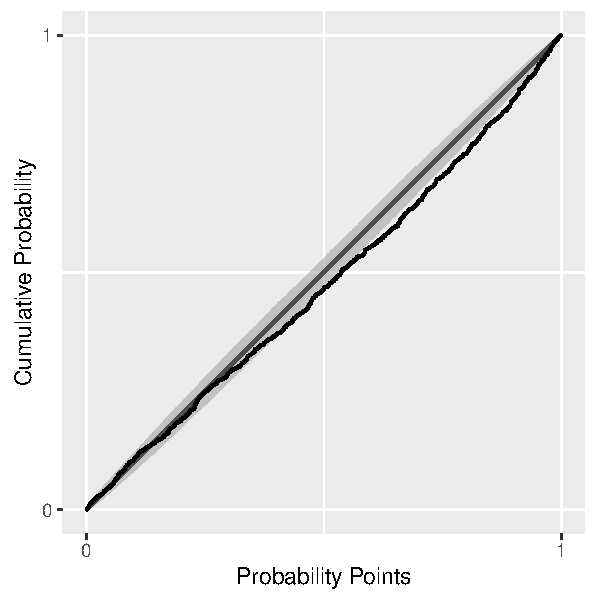
\includegraphics[width=\textwidth]{figures/sim_800_normal_-0.4_0}
  \caption{Q-Q p}
  \label{fig:mu}
\end{figure}

\begin{figure}[tbp]
  \centering
  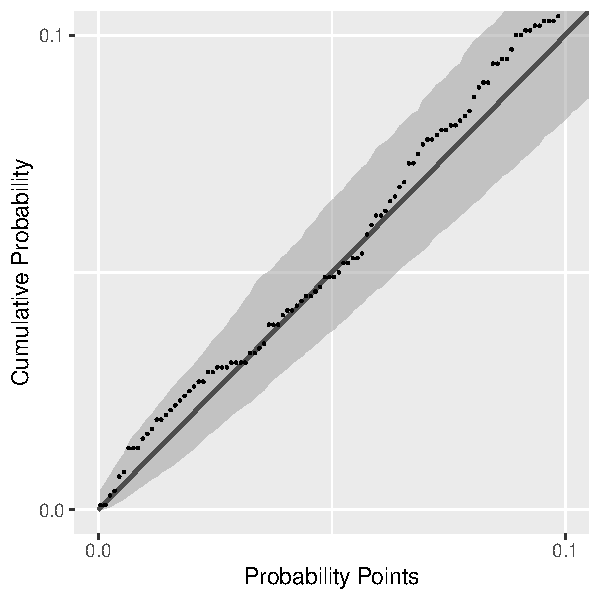
\includegraphics[width=\textwidth]{figures/zoom_800_normal_-0.4_0}
  \caption{}
  \label{fig:mu}
\end{figure}


\paragraph{Power}
We must also evaluate if this method works when $H_0$ is false. We can use
the block bootstrap KS test to test if $X_t$ is generated from some other 
distribution $G$ with some unknown $\theta$. In this scenario, if the test is 
indeed powerful,
we would ideally want $\Beta$, or the probability of rejection to be 1, but we
expect it to be generally high. Again, we must try the method with different
marginal distributions to ensure that it is robust.


\section{Real Data Analysis}

\jy{Find some real time series to test for their marginal distributions. Open
  data, for example, temperatures or stock returns or ...}

\subsection{Precipitation in Mansfield Connecticut}
Precipitation annual maximum in inches series data was retrieved from the 
National Oceanic and Atmospheric Administration.
\mc{https://hdsc.nws.noaa.gov/pfds/pfds_map_cont.html?bkmrk=ct}

\subsection{Microsoft Stock Returns}

\mc{https://www.nasdaq.com/market-activity/stocks/msft/historical}

We expect the distribution of Microsoft stock returns to have a slightly
heavier tail than the normal distribution. We can test that it is normally
distributed (which we expect to reject). Then we can try testing if it follows
the $t$ distribution with different degrees of freedoms.


\section{Concluding Remarks}
\label{sec:conclusion}





\bibliographystyle{chicago}
\bibliography{citations}


\end{document}
%%% LocalWords: nonparametric semiparametric autocorrelation ARMA
%%% Local Variables:
%%% mode: latex
%%% TeX-master: t
%%% ispell-personal-dictionary: ".aspell.en.pws"
%%% fill-column: 80
%%% eval: (auto-fill-mode 1)
%%% End: